%%%%%%%%%%%%%%%%%%%%%%%%%%%%%%%%%%%%%%%%%%%%%%%%%%%%
%%%            Text
%%% Compile the master file! 
%%% Slides template: Antonio Machicao y Priemer
%%% Author: Antonio Machicao y Priemer
%%% Title: 
%%%%%%%%%%%%%%%%%%%%%%%%%%%%%%%%%%%%%%%%%%%%%%%%%%%%



%%%%%%%%%%%%%%%%%%%%%%%%%%
%%%             Preamble's End
%%%%%%%%%%%%%%%%%%%%%%%%%%


%%%%%%%%%%%%%%%%%%%%%%%%%      
\begin{frame}
  \HUtitle
\end{frame}

\frame{
%\begin{multicols}{2}
	\frametitle{Inhaltsverzeichnis}
	\tableofcontents
	%[pausesections]
%\end{multicols}
	}

%%%%%%%%%%%%%%%%%%%%%%%%%%
%%%%%%%%%%%%%%%%%%%%%%%%%%

\nocite{Glueck&Roedel16a}
\nocite{Krifka09b}
\nocite{Loebner15a}
\nocite{Lohnstein11a}
\nocite{Meibauer&Co07a}
\nocite{MyP17a}
\nocite{Partee&Co93a}
\nocite{ZimmermannT&Sternefeld13a}


%%%%%%%%%%%%%%%%%%%%%%%%%%%%%%%%%%%
%%%%%%%%%%%%%%%%%%%%%%%%%%%%%%%%%%%
%%% Basic literature for these slides

\begin{frame}
	\frametitle{Grundlage \& empfohlene Lektüre}
	
	\dots basierend auf \citet{Freitag&MyP19a}, \citet{MyP&Kerkhof16a} und \citet{MyP&Eberle19a}
	
	\medskip
	
	\textbf{\LaTeX -Reader:}
	
	\href{https://doi.org/10.13140/RG.2.2.29299.27682}{https://doi.org/10.13140/RG.2.2.29299.27682}
	
	\begin{itemize}
		\item \textbf{obligatorisch:}
		\item[] \citet{Plungian00a}
		\item[] \citet{Salmon00a}
		\item[] \citet{Wurzel00a}
		
		\item \textbf{optional:}
		\item[] \citet[41--45]{Abramowski16a}
		\item[] \citet[Kap. 7]{Luedeling09a}
		\item[] \citet[Kap. 2, S. 29--36]{Meibauer&Co07a}
		
	\end{itemize}
	
\end{frame}

	
%%%%%%%%%%%%%%%%%%%%%%%%%%
%%%%%%%%%%%%%%%%%%%%%%%%%%
\section{Einführung}
\frame{
%\begin{multicols}{2}
\frametitle{~}
	\tableofcontents[currentsection,hidesubsections]
%\end{multicols}
}
%%%%%%%%%%%%%%%%%%%%%%%%%%

\begin{frame}%{Einführung}
\frametitle{Einführung}


\begin{itemize}
	
	\item  Aussagenlogik ist \textbf{nicht ausreichend} für eine angemessene Theorie der Bedeutung natürlicher Sprachen
	\medskip

	\item Aussagenlogik: Bezug auf \emph{elementare Aussagen}
	\medskip
	
	\item Bedeutung der \textbf{Teile} von Aussagen \ras Mengen (darauf aufbauend Relationen und Funktionen)
	

\end{itemize}

\end{frame}


%%%%%%%%%%%%%%%%%%%%%%%%%%
%%%%%%%%%%%%%%%%%%%%%%%%%%
\section{Grundbegriffe \& Notation}
\frame{
	%\begin{multicols}{2}
	\frametitle{~}
	\tableofcontents[currentsection,hidesubsections]
	%\end{multicols}
}
%%%%%%%%%%%%%%%%%%%%%%%%%%

\begin{frame}{Grundbegriffe \& Notation}

\textbf{umgangsprachlicher} Begriff \obj{Menge} $\neq$ \textbf{mathematischer} Begriff \obj{Menge}

\vspace{.5cm}

\begin{minipage}{.40\textwidth}
	\begin{figure}
		\begin{center}
			\includegraphics[scale=.5]{pictures/Georg-Cantor-1894}
		\end{center}	
		\caption{Georg Cantor (ca.\ 1894)}
	\end{figure}
\end{minipage}
%%
\begin{minipage}{.55\textwidth}

\centering

\begin{block}{Mengenlehre}
	Die Mengenlehre wurde gegen Ende des 19.\ Jahrhunderts von dem Mathematiker \textbf{Georg Cantor} als theoretische Basis der Mathematik entwickelt. Der Grundgedanke war, eine \textbf{elementare, einfache und konsistente Theorie} zu schaffen, auf deren Grundlage sich \textbf{die gesamte Mathematik} aufbauen ließe.
\end{block}

\end{minipage}
	
\end{frame}


%%%%%%%%%%%%%%%%%%%%%%%%%%
%%%%%%%%%%%%%%%%%%%%%%%%%%
\subsection{Definition}
%\frame{
%\begin{multicols}{2}
%\frametitle{~}
%	\tableofcontents[currentsection]
%\end{multicols}
%}
%%%%%%%%%%%%%%%%%%%%%%%%%%

\begin{frame}{Definition}

\begin{block}{Mengen (engl. \obj{set})}
	\textbf{Abstrakte Zusammenfassung} bestimmter \textbf{wohlunterschiedener} Objekte unserer Anschauung oder unseres Denkens zu einem Ganzen
\end{block}

\begin{itemize}
\item \textbf{abstrakt:} nicht \alert{notwendigerweise} physische Objekte 

\end{itemize}

\pause

\ea A $:= \{Liebe, Hass, Verbitterung\}$

\ex B $:= \{Tisch, Stuhl, Schrank\}$

\ex C $:= \{BND, Flasche, Verzweiflung, Schweinsteiger\}$
\z 


\end{frame}


%%%%%%%%%%%%%%%%%%%%%%%%%%
%%%%%%%%%%%%%%%%%%%%%%%%%%
\subsection{Arten von Mengen}
%\frame{
%\begin{multicols}{2}
%\frametitle{~}
%	\tableofcontents[currentsection]
%\end{multicols}
%}
%%%%%%%%%%%%%%%%%%%%%%%%%%

\begin{frame}{Arten von Mengen}

\begin{itemize}
	\item \textbf{Kleine} Mengen
	\ea A $:=$ Menge der Wochentage
	\z 
	
	\item \textbf{Große} Mengen
	\ea B $:=$ Menge aller Bücher auf der Welt
	\z 
	
	\item A \& B sind \textbf{endliche} Mengen
%	\medskip
	
	\item \textbf{unendliche} Menge
	\ea C $:=$ Menge der natürlichen Zahlen
	\z 
	
	
	\item \textbf{Einermenge} (engl. \obj{singleton}): Menge mit nur einem Element
	\ea D $:= \{Burrito\}$
	\z 
	
	\item Menge ohne Elemente (\textbf{leere Menge}): $\emptyset$ auch $\{\}$ 
	
	\item \textbf{Menge} mit der leere Menge: $\{ \emptyset \}$ auch $\{\{\}\}$ 
	
\end{itemize}

\end{frame}


%%%%%%%%%%%%%%%%%%%%%%%%%%
%%%%%%%%%%%%%%%%%%%%%%%%%%
\subsection{Prädikatsnotation}
%\frame{
%\begin{multicols}{2}
%\frametitle{~}
%	\tableofcontents[currentsection]
%\end{multicols}
%}
%%%%%%%%%%%%%%%%%%%%%%%%%%

\begin{frame}{Prädikatsnotation}

\begin{itemize} 
	\item \textbf{Notation:} $\{$Variable $|$  Beschreibung der Variable $\}$
\end{itemize}


\pause 

\settowidth\jamwidth{(unendliche Menge)} 
\ea $\{x | x$ ist ein Grundvokal$\}$ 
\jambox{(kleine Menge)}

\pause

\ex $\{x | x$ ist eine natürliche Zahl und $1 \leq x \leq 1.000.000 \}$ 
\jambox{(große Menge)}

\pause

\ex $\{x | x$ ist eine natürliche Zahl$\}$ 
\jambox{(unendliche Menge)} 

\z 


Lies: \gqq{die Menge aller $x$, sodass $x$ ist ein $\langle$\emph{Beschreibung}$\rangle$}

\end{frame}


%%%%%%%%%%%%%%%%%%%%%%%%%%
%%%%%%%%%%%%%%%%%%%%%%%%%%
\subsection{Kardinalität}
%\frame{
%\begin{multicols}{2}
%\frametitle{~}
%	\tableofcontents[currentsection]
%\end{multicols}
%}
%%%%%%%%%%%%%%%%%%%%%%%%%%

\begin{frame}{Kardinalität}

\begin{itemize}
	\item \textbf{Kardinalität:} Elementenanzahl einer Menge
	
	\item \textbf{Notation:} $|$A$| = 5$ oder $\#($A$)$ = 5 oder $\# \{$a, b, c, d, e$\} = 5$
\end{itemize}

\ea A $:= \{a, e, i, o, u\}$ \hfill (Menge der 5 Grundvokale)

\ex B $:= \{a, e, i, \{o, u\}\}$ \hfill (Menge mit 4 Elementen)

\z 
\end{frame}


%%%%%%%%%%%%%%%%%%%%%%%%%%
%%%%%%%%%%%%%%%%%%%%%%%%%%
\subsection{Leere Menge}
%\frame{
%\begin{multicols}{2}
%\frametitle{~}
%	\tableofcontents[currentsection]
%\end{multicols}
%}
%%%%%%%%%%%%%%%%%%%%%%%%%%

\begin{frame}{Leere Menge}

	\begin{multicols}{2}
		
\begin{itemize}
	\item Die Kardinalität einer Menge ist die Anzahl von Elementen dieser Menge
	
	\ea $\#\{a\} = 1$
	\z 

\pause 	

	\item Wenn die \textbf{leere Menge als Element} in einer Menge aufgeschrieben wird, dann \dots 
	
	\ea $\#\{\emptyset , a\} = 2$
	\z 

\pause 

	\item Es gilt:
	
	\ea $\emptyset \in \{ \emptyset , a \}$
	\ex $\emptyset \subseteq \{ \emptyset , a \}$
	\ex $\emptyset \notin \{ a \}$
	\ex $\emptyset \subseteq \{ a \}$ 
	\z 
	(weil \textbf{alle Elemente in der $\emptyset$ auch Elemente der anderen Menge} sind)

\pause 
	
	\item Zur Kardinalität:

	\ea $\#\{\emptyset , \{ \emptyset \} \} = 2$
	\ex $\#\{\emptyset , \emptyset \} = 1$
	\ex $\#\{ \} = 0$ oder $\#\emptyset = 0$
	\z 

\end{itemize}	

\end{multicols}	

\end{frame}


%%%%%%%%%%%%%%%%%%%%%%%%%%
%%%%%%%%%%%%%%%%%%%%%%%%%%
\subsection{Venn-Diagramm}
%\frame{
%\begin{multicols}{2}
%\frametitle{~}
%	\tableofcontents[currentsection]
%\end{multicols}
%}
%%%%%%%%%%%%%%%%%%%%%%%%%%

\begin{frame}{Venn-Diagramm}
	
\begin{minipage}{.48\textwidth}
	
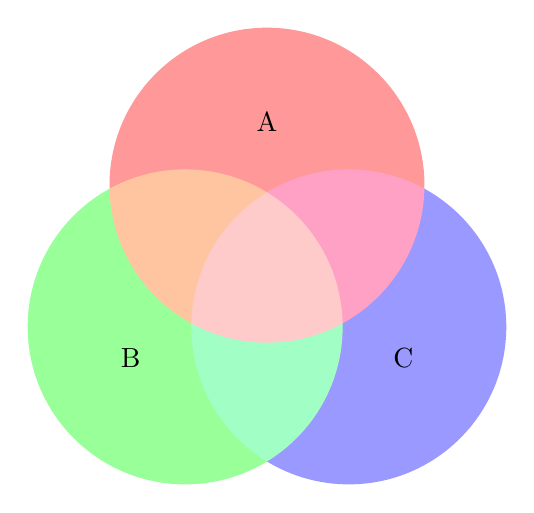
\begin{tikzpicture}

\begin{scope}[blend group=soft light]

	\fill[red!40!white]   (90:1.2) circle (2);
	\fill[green!40!white] (210:1.2) circle (2);
	\fill[blue!40!white]  (330:1.2) circle (2);

\end{scope}

	\node at (90:2)    {A};
	\node at (210:2)    {B};
	%	\node at (210:1)    {a b c};
	\node at (330:2)    {C};
	%	\node [font=\Large] {\LaTeX};

\end{tikzpicture}
	
\end{minipage}
%%
%%
\begin{minipage}{.48\textwidth}

\begin{figure}
	\centering
	\begin{center}
		\includegraphics[scale=.5]{pictures/John-Venn}
	\end{center}	
	\caption{John Venn}
\end{figure}
		
\end{minipage}	
	
\end{frame}


%%%%%%%%%%%%%%%%%%%%%%%%%%
%%%%%%%%%%%%%%%%%%%%%%%%%%
%\section{XY}
%%\frame{
%%\begin{multicols}{2}
%%\frametitle{~}
%%	\tableofcontents[currentsection]
%%\end{multicols}
%%}
%%%%%%%%%%%%%%%%%%%%%%%%%%
%
%\begin{frame}{XY}
%
%\begin{itemize}
%	\item XY
%\end{itemize}
%
%\end{frame}

